\section{Crossing boundaries}

\begin{frame}[c]
  \frametitle{Of standards\ldots{}}
  \begin{figure}
    \centering
    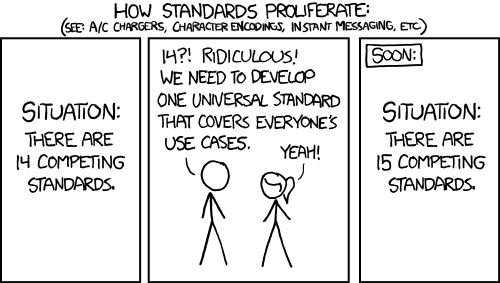
\includegraphics[width=0.6\linewidth]{standards}
    \caption{http://xkcd.com/927/}
  \end{figure}
\end{frame}

\begin{frame}[c]
  \frametitle{\ldots{}and ABIs}\pause{}
  \begin{itemize}
    \item{Think API on \textbf{B}inary level}\pause{}
    \item{Covers}\pause{}
      \begin{itemize}
        \item{Instruction set}\pause{}
        \item{Calling conventions}\pause{}
        \item{Names of things}\pause{}
      \end{itemize}
    \item{C++ does \textbf{NOT} specify a standard ABI}
  \end{itemize}
\end{frame}

\begin{frame}[c]
  \frametitle{An introductory example - overview}
  \begin{figure}
    \centering
    \includegraphics[width=\linewidth]{the_problem}
  \end{figure}
\end{frame}

\begin{frame}[c]
  \frametitle{An introductory example - fancy.cpp}
  \inputminted{cpp}{code/fancy1/fancy.cpp}
\end{frame}

\begin{frame}[c]
  \frametitle{An introductory example - fancy\_doge.cpp}
  \inputminted{cpp}{code/fancy1/fancy_doge.cpp}
\end{frame}

\begin{frame}[c]
  \frametitle{An introductory example - fancy\_sloth.cpp}
  \inputminted{cpp}{code/fancy1/fancy_sloth.cpp}
\end{frame}

\begin{frame}[c]
  \frametitle{Looks good to me!}
  \begin{centering}
    \Large{What could possibly go wrong?}
  \end{centering}
\end{frame}

\begin{frame}[c]
  \frametitle{This error is so fancy, I need a second monocle!}
  \only<1>{
    \inputminted[breaklines]{text}{code/fancy1/log/fancy_sloth.log}
  }
  \only<2>{
    \begin{figure}
      \centering
      
\includegraphics[width=0.6\linewidth]{why}
    \end{figure}
  }
\end{frame}

\begin{frame}[c]
  \frametitle{There is no single STL}
    \begin{figure}
      \centering
      \includegraphics[width=\linewidth]{the_problem_with_stdlib}
    \end{figure}
\end{frame}

\begin{frame}[c]
  \frametitle{It is not just libraries!}\pause{}
  \begin{itemize}
    \item{GCC changed its C++ ABI from 2.95 to 3.0}\pause{}
    \item{\ldots{}and again from 3.0 to 3.1}\pause{}
    \item{\ldots{}and yet again from 3.1 to 3.2}\pause{}
    \item{\ldots{}and again with version 3.4}\pause{}
    \item{\ldots{}and pretty much again with version 5.1}
  \end{itemize}
\end{frame}

\begin{frame}[c]
  \frametitle{But\ldots{} what can we do?}\pause
  \begin{itemize}
    \item{Use C}\pause{}
    \item{seriously!}\pause{}
    \item{C has extremely stable ABIs}\pause{}
    \item{Use C as the "frontend"}\pause{}
    \item{C++ under the hood}
  \end{itemize}
\end{frame}

\begin{frame}[c]
  \frametitle{Introducing the Hourglass Interface}
    \begin{figure}
      \centering
      \includegraphics[width=\linewidth]{hourglass}
    \end{figure}
\end{frame}

\begin{frame}[c]
  \frametitle{What is that?}\pause{}
  \begin{itemize}
    \item{Full C++ on the bottom-end}\pause
    \item{LanguageXYZ on the upper-end}\pause
    \item{Stable C interface in between}\pause
    \item{Excellent talk by Stefanus DuToit @ CppCon 2014}
      \begin{itemize}
        \item{\url{https://www.youtube.com/watch?v=PVYdHDm0q6Y}}
      \end{itemize}
  \end{itemize}
\end{frame}

\begin{frame}[c]
  \frametitle{Back to our example}
  \begin{figure}
    \centering
    \includegraphics[width=\linewidth]{the_problem}
  \end{figure}
\end{frame}

\begin{frame}[c]
  \frametitle{Its not that simple anymore}
  \begin{figure}
    \centering
    \includegraphics[width=0.55\linewidth]{hourglass_architecture}
  \end{figure}
\end{frame}

\begin{frame}[c]
  \frametitle{Lets look at some code - fancy.h}
  \inputminted[firstline=4,lastline=15]{cpp}{code/fancy2/fancy.h}
\end{frame}

\begin{frame}[c]
  \frametitle{Lets look at some code - fancy.cpp}
  \inputminted[firstline=4]{cpp}{code/fancy2/fancy.cpp}
\end{frame}

\begin{frame}[c]
  \frametitle{Lets look at some code - fancy\_lib.hpp}
  \inputminted[firstline=4,lastline=12]{cpp}{code/fancy2/fancy_lib.hpp}
\end{frame}

\begin{frame}[c]
  \frametitle{Lets look at some code - fancy\_lib.cpp}
  \inputminted[firstline=3]{cpp}{code/fancy2/fancy_lib.cpp}
\end{frame}

\begin{frame}[c]
  \frametitle{What is important?}\pause{}
  \begin{itemize}
    \item{No function overloading in C}\pause{}
    \item{No namespaces in C}\pause{}
    \item{No exceptions in C}\pause{}
    \item{Use \mintinline{cpp}{extern "C"} to prevent name-mangling}\pause{}
    \item{(Optionally) Use visibility specifiers}
  \end{itemize}
\end{frame}

\begin{frame}[c]
  \frametitle{Speaking foreign languages - fancy\_gopher.go}
  \inputminted[firstline=3,lastline=13]{go}{code/fancy2/fancy_gopher.go}
\end{frame}

\begin{frame}[c]
  \frametitle{Speaking foreign languages - fancy\_python.py}
  \inputminted[firstline=3,lastline=10]{python}{code/fancy2/fancy_python.py}
\end{frame}

\begin{frame}[c]
  \frametitle{But I want classes!}\pause{}
  \begin{itemize}
    \item{\mintinline{cpp}{struct}s cannot have member functions in C}\pause{}
    \item{But we have opaque pointers}\pause{}
    \item{Sounds familiar?}
  \end{itemize}
\end{frame}

\begin{frame}[c]
  \frametitle{A box of \mintinline{cpp}{int}s}
    \begin{figure}
      \centering
      \includegraphics[width=0.6\linewidth]{box}
    \end{figure}
\end{frame}

\begin{frame}[c]
  \frametitle{A box of \mintinline{cpp}{int}s}\pause{}
  \begin{itemize}
    \item{Create a box of a fixed size}\pause{}
    \item{Push values inside}\pause{}
    \item{Pop them back out}\pause{}
    \item{Important: Destroy the box!}
  \end{itemize}
\end{frame}


\begin{frame}[c]
  \frametitle{C with classes - box.h}
  \only<1>{
    \inputminted[firstline=14,lastline=14]{c}{code/box/box.h}
  }
  \only<2>{
    \inputminted[fontsize=\scriptsize,firstline=14,lastline=26]{c}{code/box/box.h}
  }
\end{frame}

\begin{frame}[c]
  \frametitle{C with classes - box.cpp}
  \inputminted[firstline=6,lastline=9]{c}{code/box/box.cpp}
\end{frame}

\begin{frame}[c]
  \frametitle{C with classes - box\_impl.hpp}
  \inputminted[fontsize=\scriptsize,firstline=8,lastline=19]{c}{code/box/box_impl.hpp}
\end{frame}

\begin{frame}[c]
  \frametitle{C with classes - cbox.c}
  \inputminted[fontsize=\scriptsize,firstline=7,lastline=17]{c}{code/box/cbox.c}
\end{frame}

\begin{frame}[c]
  \frametitle{C with classes - cppbox.cpp}
  \inputminted[firstline=5,lastline=10]{c}{code/box/cppbox.cpp}
\end{frame}

\begin{frame}[c]
  \frametitle{Going the extra mile - gobox.bo}
  \only<1>{
    \inputminted[firstline=3,lastline=14]{c}{code/box/gobox.go}
  }
  \only<2>{
    \inputminted[firstline=16,lastline=26]{c}{code/box/gobox.go}
  }
  \only<3>{
    \inputminted[firstline=28,lastline=35]{c}{code/box/gobox.go}
  }
  \only<4>{
    \inputminted[firstline=37,lastline=46]{c}{code/box/gobox.go}
  }
  \only<5>{
    \inputminted[firstline=48]{c}{code/box/gobox.go}
  }
\end{frame}

\begin{frame}[c]
  \frametitle{What is worth noting}\pause{}
  \begin{itemize}
    \item{It is basically PIMPL for C}\pause{}
    \item{Exceptions do not propagate well}\pause{}
    \item{You need to manage the memory}\pause{}
    \item{You need to define "contracts"}
  \end{itemize}
\end{frame}
